\documentclass[10pt,a4paper]{article}
\usepackage{amsmath,amssymb,amsthm,graphicx}
\usepackage{mathtools,tikz,hyperref}
\usetikzlibrary{positioning,shapes,decorations.pathreplacing}
\newtheorem{theorem}{Theorem}
\newtheorem{lemma}[theorem]{Lemma}
\newtheorem{claim}[theorem]{Claim}
\newtheorem{fact}[theorem]{Fact}
\newtheorem{observation}[theorem]{Observation}
\theoremstyle{definition}
\newtheorem{definition}[theorem]{Definition}
\newtheorem{remark}[theorem]{Remark}
\newcommand{\bra}[1]{\{#1\}}
\newcommand{\pmone}{\bra{-1,1}}
\newcommand{\R}{\mathbb R}
\newcommand{\E}{\mathbb E}
\newcommand{\wh}{\widehat}
\newcommand{\eps}{\epsilon}
\newcommand{\abs}[1]{\lvert#1\rvert}
\newcommand{\adeg}{\widetilde{\mathrm{deg}}}
\newcommand{\asnorm}[2]{\|\widehat{#1}\|_{1,#2}}
\newcommand{\snorm}[1]{\|\widehat{#1}\|_1}
\newcommand{\ADD}{\mathsf{ADDR}}
\newcommand{\HADD}{\mathsf{HADD}}
\newcommand{\IND}{\mathsf{IND}}
\newcommand{\PARITY}{\mathsf{PARITY}}
\newcommand{\what}{\textnormal{selector}}
\DeclareMathOperator*{\Exp}{\mathbb E}
\AtBeginDocument{\author{Sourav Chakraborty, Arkadev Chattopadhyay\\Nikhil S. Mande, Manaswi Paraashar}}
\title{A total XOR-composed function requiring logarithmic overhead in bounded-error quantum query-to-communication simulation}
\author{Sourav Chakraborty, Arkadev Chattopadhyay, Nikhil S. Mande, Manaswi Paraashar}
\date{doi:10.4230/LIPIcs.CCC.2020.32; CC BY 3.0 Unported}
\begin{document}
\maketitle
\noindent\textit{Editorial note.} Editable transcription of formally published CC BY3.0 text. Nonexclusive native private only; formal corrections in addressing definition, approximate-norm notation, query proof indices/lowerbound and the full target-degree/Fourier argument transcribed from official pages7–12. Formally printed author parameters and displayed spectral-norm consequences retained without mathematical repair. Figure1 author TikZ flattened and label moved aftercaption. All source-local proof retained; standard cited prerequisites not reproved. No added entanglement convention: formal bounded-error model definition retained. Theorems4/Lemma6/parameterbranches/directconsequences uncounted supports. Production andmaterialvalidation onlyYupeng; rootownscompilation.\par\medskip
\noindent\textit{Allowed standard prerequisites (editorial).}\begin{itemize}
\item Bernstein-Vazirani and Grover algorithms, parity query lowerbound, Lee-Shraibman communication lowerbound. Authors cited standard results; full source-local addressing spectral-norm lifting proof retained
\end{itemize}\medskip
\setcounter{theorem}{2}
\begin{theorem}[Main Theorem]\label{thm: extmain}
For any constant $0 < \delta < 1$, there exists a total function $F : \pmone^n \to \pmone$ for which $Q(F) = \Theta(n^{\delta})$ and 
\[
Q^{cc}(F \circ \oplus) = \Theta(Q(F) \log n).
\]
\end{theorem}

\section*{Selected author context and supporting statements}
Recall a standard way to derive a communication problem from a function $f:\pmone^n\to\pmone$. Each input bit is encoded between Alice and Bob using a binary primitive $\bullet:\pmone\times\pmone\to\pmone$, giving $(f\circ\bullet)(x,y)=f(\bullet(x_1,y_1),\ldots,\bullet(x_n,y_n))$, where $x,y$ are the respective $n$-bit inputs.
\setcounter{theorem}{0}
\begin{theorem}[\cite{BCW98}]\label{thm: qtm_sim_log_loss}
For any Boolean function $f : \pmone^n \to \pmone$, we have 
\[
Q^{cc}\big(f \circ \bullet\big) = O\big(Q(f)\cdot \log n\big),
\]
where $\bullet$ is either $\wedge$ or $\oplus$.
\end{theorem}
Here $Q(f)$ denotes bounded-error quantum query complexity and $Q^{cc}$ denotes bounded-error quantum communication complexity.
\setcounter{theorem}{3}
\begin{theorem}\label{thm: wtdeg}
For any constant $0 < \delta < 1$, there exists a total function $F : \pmone^n \to \pmone$ for which $Q(F) = \Theta(n^{\delta})$ and 
\[
    \log\big( \asnorm{F}{1/3} \big)= \Theta(Q(F) \log n).
\]
\end{theorem}
\setcounter{theorem}{5}
\begin{lemma}[extending \cite{CM17}]\label{lem: lifting} \label{lemma:degree-norm-lifting}
Let $t > 1$ be any integer, $\ADD_{m,t}$ be any (partial) addressing function and $f : \pmone^n \to \pmone$ be any function. Then,
\[
   \log\left(\asnorm{f^{\ADD_{m,t}}}{1/3}\right) = \Omega\left(\adeg(f) \log t\right).
\]
\end{lemma}

\setcounter{section}{1}
\setcounter{theorem}{9}
\section{Preliminaries}\label{sec: prelims}
For any positive integer $n$, we denote the set $\{1, \dots, n\}$ by $[n]$. For $d \leq n$ we use the notation $\binom{n}{\leq d} = \binom{n}{0} + \cdots + \binom{n}{d}$. Note that $\binom{n}{\leq d} < (n+1)^d$.

In this section we review the necessary preliminaries.  We first review some basics of Fourier analysis on the Boolean cube.
Consider the vector space of functions from $\pmone^n$ to $\R$, equipped with an inner product defined by
\[
\langle f, g \rangle := \E_{x \in \pmone^n}[f(x)g(x)] = \frac{1}{2^n}\sum_{x \in \pmone^n}f(x)g(x).
\]
for every $f,g: \pmone^n \rightarrow \R$. For any set $S \subseteq [n]$, define the associated \emph{parity} function $\chi_S$ by $\chi_S(x) = \prod_{i \in S}x_i$. The set of parity functions $\bra{\chi_S : S \subseteq [n]}$ form an orthonormal basis for this vector space.  Thus, every function $f : \pmone^n \to \R$ has a unique multilinear expression as
\[
f = \sum_{S \subseteq [n]}\wh{f}(S)\chi_S.
\]
We also use $\PARITY_n$ to denote $\chi_{[n]}:\pmone^n\to\pmone$.
The coefficients $\bra{\wh{f}(S) : S \subseteq [n]}$ are called the \emph{Fourier coefficients} of $f$.
\begin{fact}[Parseval's Identity]\label{fact: parseval}
For any function $f : \pmone^n \to \R$,
\[
    \sum_{S \subseteq [n]}\wh{f}(S)^2 = \frac{\sum_{x \in \pmone^n}f(x)^2}{2^n}.
\]
\end{fact}

\begin{definition}[Spectral Norm]\label{defn: wt}
For any function $f : \pmone^n \to \R$, define its \emph{spectral norm}, which we denote $\snorm{f}$, to be the sum of absolute values of the Fourier coefficients of $f$.  That is,
\[
\snorm{f} : = \sum_{S \subseteq [n]}\abs{\wh{f}(S)}.
\]
\end{definition}

\begin{definition}[Hadamard Codeword]\label{defn: hcwd}
If a $\ell$-bit string $(x_1, \dots, x_{\ell}) \in \pmone^\ell$ (alternatively, view the indices of $x$ as subsets of $[\log\ell]$) is of the form $x_S = \prod_{i \in S}z_i$ for all $S \subseteq [\log \ell]$ for some $z \in \pmone^{\log \ell}$, then define such an $x = x_1 \dots x_\ell$ to be the \emph{$\ell$-bit Hadamard codeword} $h(z)$ of the $(\log \ell)$-bit string $z$.
\end{definition}

\subsection{Addressing functions}
\begin{definition}[$(m,k)$-addressing function]\label{defn: add}
We define a (partial) function $f:\pmone^{m+k} \rightarrow \bra{-1, 1, \star}$ to be an \emph{$(m,k)$-addressing function} if there exists $g : \pmone^m \to \bra{[k] \cup \star}$ such that 
\begin{itemize}
    \item $f(x_1, \dots, x_m, y_1, \dots, y_{k}) = y_{g(x_1, \dots, x_m)}$ if $g(x_1, \dots, x_m) \in [k]$, and $f(x_1, \dots, x_m, y_1, \dots, y_{k}) = \star$ otherwise.
    \item For all $j \in [k]$, there exists $(x_1, \dots, x_m) \in \pmone^m$ such that $g(x_1, \dots, x_m) = j$.
\end{itemize}

We call the variables $\{x_1, \dots, x_m\}$ the \emph{address variables} and the variables $\{y_{1}, \dots, y_{k}\}$ the \emph{target variables}.  The function $g$ is called the $\what$ function of $f$.
\end{definition}

\begin{definition}[Indexing Function]
The Indexing function, which we denote by $\IND_k$, is a $(k, 2^k)$-addressing function defined by $\IND(x_1, \dots, x_k, y_1, \dots, y_{2^k}) = y_{\textnormal{bin}(x)}$, where $\textnormal{bin}(x)$ denotes the integer represented by the binary string $x_1, \dots, x_k$.
\end{definition}

\begin{definition}[Composition with addressing functions]\label{defn: addcomp}
For any function $f : \pmone^n \to \pmone$ and an $(m, k)$-addressing function $\ADD$, define the (partial) function $f^{\ADD} : \pmone^{n (m + k)} \to \bra{-1, 1, \star}$ by
\[
f^{\ADD}(x_1, y_1, \dots, x_n, y_n) = 
\begin{cases}
f(\ADD(x_1, y_1), \dots, \ADD(x_n, y_n)) & \text{if~} \ADD(x_i, y_i) \in \pmone \text{~for all~} i \in [n]\\
\star & \text{otherwise}.
\end{cases}
\]
where $x_i \in \pmone^{m}$ and $y_i \in \pmone^k$ for all $i \in [n]$.
\end{definition}

\begin{definition}[Hadamard Addressing Function]\label{defn: hadd}
We define the \emph{Hadamard addressing function}, which we denote $\HADD_\ell : \pmone^{2\ell} \to \bra{-1, 1, \star}$, as follows.
Fix an arbitrary order on the $\ell$-many Hadamard codewords of $(\log \ell)$-bit strings, say $w_1, \dots, w_\ell$.  Define the selector function of $\HADD_\ell$ by
\begin{align*}
g(x) & =\begin{cases}
i & \text{if~} x = w_i \text{~for some~} i \in [\ell]\\
\star & \text{otherwise}.
\end{cases}
\end{align*}
Note that $\HADD_\ell$ is an $(\ell, \ell)$-addressing function.
\end{definition}

\subsection{Polynomial approximation}

\begin{definition}[Approximate Degree]\label{defn: adeg}
The \emph{$\eps$-approximate degree} of a function $f : \pmone^n \to \bra{-1, 1, \star}$, denoted by $\adeg_\eps(f)$ is defined to be the minimum degree of a real polynomial $p : \pmone^n \to \R$ that satisfies $\abs{p(x) - f(x)} \leq \eps$ for all $x \in \pmone^n$ for which $f(x) \in \pmone$.\footnote{When dealing with partial functions, another notion of approximation is sometimes considered, where the approximating polynomial $p$ is required to have bounded values even on the non-promise inputs of $f$.  For the purpose of this paper, we do not require this constraint.} That is,
\[
\adeg_\eps(f):=\min\left\{d:\begin{array}{l}\deg(p)\leq d,\quad |p(x)-f(x)|\leq\epsilon\\\text{for all }x\in\pmone^n\text{ for which }f(x)\in\pmone\end{array}\right\}.
\]
\end{definition}
Henceforth, we will use the notation $\adeg(f)$ to denote $\adeg_{1/3}(f)$.

\begin{definition}[Approximate Spectral Norm]\label{defn: awt}
The \emph{approximate spectral norm} of a function  $f : \pmone^n \to \{-1,1,\star\}$, denoted by $\asnorm{f}{\epsilon}$ is defined to be the minimum spectral norm of a real polynomial $p : \pmone^n \to \R$ that satisfies $\abs{p(x) - f(x)} \leq \eps$ for all $x \in \pmone^n$ for which $f(x) \in \pmone$.
\[
\asnorm{f}{\epsilon}:=\min\left\{\snorm{p}:\begin{array}{l}|p(x)-f(x)|\leq\epsilon\\\text{for all }x\in\pmone^n\text{ for which }f(x)\in\pmone\end{array}\right\}.
\]
\end{definition}
\begin{lemma}[\cite{BNRW07}]\label{lem: asnormequiv} 
Let $f:\pmone^n \to \pmone$ be a total function. Then for all constants $0 < \delta, \eps < 1$ we have $\adeg_\eps(f) = \Theta(\adeg_\delta(f))$. The constant hidden in the $\Theta$ notation depends on $\delta$ and $\eps$.
\end{lemma}

The following is a standard upper bound on the approximate spectral norm of a Boolean function in terms of its approximate degree.
\begin{claim}\label{claim: adegnaivelb}
For all total functions $f : \pmone^n \to \pmone$, we have 
\[
\log \asnorm{f}{1/3} = O(\adeg(f) \log n).
\]
\end{claim}
\begin{proof}
Let $d$ denote the approximate degree of $f$.  Take any 1/3-approximating polynomial of degree $d$, say $p$, to $f$.  Then,
\begin{align*}
    \sum_{S \subseteq [n]} \abs{\wh{p}(S)} & \leq \sqrt{\binom{n}{\leq d}} \cdot \sqrt{\sum_{S: |S| \leq d}\wh{p}(S)^2} \leq 4/3 \cdot (n+1)^{d/2} = 2^{O(d \log n)},
\end{align*}

where the first inequality follows by the Cauchy-Schwarz inequality, the second inequality follows by Parseval's identity (Fact~\ref{fact: parseval}) and the fact that the absolute value of $p$ is at most $4/3$ for any input $x \in \pmone^n$.
\end{proof}

It is easy to exhibit functions $f : \pmone^n \to \pmone$ such that $\log \asnorm{f}{1/3} = \Omega(\adeg(f))$.  Bent functions satisfy this bound, for example.

Building upon ideas in~\cite{KP97}, the approximate spectral norm of $f \circ \IND_1$ was shown to be bounded below by $2^{\Omega(\adeg(f))}$ in~\cite{CM17}.
\begin{theorem}[\cite{CM17}]
Let $f:\pmone^n \rightarrow \pmone$ be any function. Then $\asnorm{f\circ\IND_1}{1/3} \geq 2^{c \cdot \adeg_{2/3}(f)}$ for any constant $c < 1 - 3/\adeg_{2/3}(f)$.
\end{theorem}

\subsection{Communication complexity}
The classical model of communication complexity was introduced by Yao in~\cite{Yao79}. In this model two parties, say Alice and Bob, wish to compute a function whose output depends on both their inputs. Alice is given an input $x \in \mathcal{X}$, Bob is given $y \in \mathcal{Y}$, and they want to jointly compute the value of a given function $F(x,y)$ by communicating with each other.  Alice and Bob individually have unbounded computational power and the number of bits communicated is the resource we wish to minimize. Alice and Bob communicate using a \emph{protocol} that is agreed upon in advance. In the randomized model, Alice and Bob have access to unlimited public random bits and the goal is to compute the correct value of $F(x,y)$ with probability at least $2/3$ for all inputs $(x,y) \in \mathcal{X} \times \mathcal{Y}$. The \emph{bounded-error randomized communication complexity} of a function $F$, denoted $R^{cc}(F)$, is the number of bits that must be communicated in the worst case by any randomized protocol to compute the correct value of the function $F(x,y)$, with probability at least $2/3$, for every $(x,y) \in \mathcal{X} \times \mathcal{Y}$.

The quantum model of communication complexity was introduced by Yao in~\cite{Yao93}. 
We refer the reader to the survey~\cite{Wolf02} for details. The \emph{bounded-error quantum communication complexity} of a function $F$, denoted $Q^{cc}(F)$ is the number of bits that must be communicated by any quantum communication protocol in the worst case to compute the correct value of the function $F(x,y)$, with probability at least $2/3$, for every $(x,y)$ in domain of $F$. Buhrman, Cleve and Wigderson~\cite{BCW98} observed a quantum simulation theorem, which gives an upper bound on the bounded-error quantum communication complexity of a composed function of the form $f \circ \wedge$ or $f \circ \oplus$ in terms of the bounded-error quantum query complexity of $f$ (see Theorem~\ref{thm: qtm_sim_log_loss}).

Lee and Shraibman~\cite{LS09} showed that the bounded-error quantum communication complexity of $f \circ \oplus$ is bounded below by the logarithm of the approximate spectral norm of $f$. Also see~\cite{CM17} for an alternate proof.
\begin{theorem}[\cite{LS09}]\label{thm: LS}
For any Boolean function $f : \pmone^n \to \pmone$,
\[
Q^{cc}(f \circ \oplus) = \Omega(\log \asnorm{f}{1/3}).
\]
\end{theorem}




\section{Proof of Theorem~\ref{thm: extmain}}\label{sec: main}
In this section, we prove Theorem~\ref{thm: extmain}.  We first formally define the function we use.

\subsection{Definition of the function}\label{sec: Fdefn}
If $\delta < 1/2$, then ignore the last $n - 2n^{2\delta}$ bits of the input, and define the following function on the first $2n^{\delta}$ bits of the input. The same argument as in Sections~\ref{sec: upper} and~\ref{sec: lower} give the required bounds for Theorem~\ref{thm: extmain} and Theorem~\ref{thm: wtdeg}.
Hence, we may assume without loss of generality that $\delta \geq 1/2$.

Define the partial function $f : \pmone^n \to \bra{-1, 1, \star}$ by $f = \PARITY_{n^{\delta}/2}^{\HADD_{n^{1 - \delta}}}$.
Define $F$ to be the completion of $f$ that evaluates to $-1$ on the non-promise domain of $f$ (see Figure~\ref{fig: cexample}).




\begin{figure}[htbp]
\begin{center}
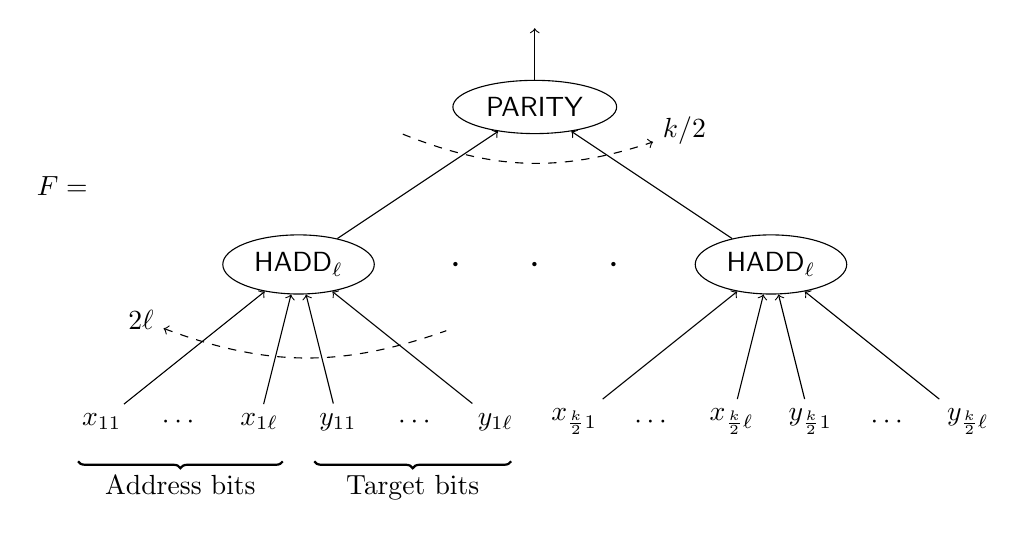
\begin{tikzpicture}

\tikzstyle{gate}=[ellipse,draw=black]
\tikzstyle{input}=[]
\node(hdef) at (-6, -1){$F = $};
\node[gate] (root) at (0,0) {$\mathsf{PARITY}$};
\node[gate] (c1) at (-3,-2) {$\mathsf{HADD}_\ell$};
\node[gate] (cn) at (3,-2) {$\HADD_{\ell}$};
\node (dummy1) at (-1.8, -0.3) {};
\node (dummy2) at (1.9, -0.3) {$k/2$};
\draw[->, dashed] (dummy1) edge [bend right = 20] (dummy2);

\node (dummy3) at (-5, -2.7) {$2\ell$};
\node (dummy4) at (-1, -2.8) {};
\draw[<-, dashed] (dummy3) edge [bend right = 20] (dummy4);


\node[input] (x8) at (1,-2) {$\boldsymbol{\cdot}$};
\node[input] (x19) at (-1,-2) {$\boldsymbol{\cdot}$};
\node[input] (x419) at (0,-2) {$\boldsymbol{\cdot}$};

\node[input] (x11) at (-5.5,-4) {$x_{11}$};
\node[input] (x123) at (-4.5,-4) {$\cdots$};
\node[input] (x1f) at (-3.5,-4) {$x_{1\ell}$};
\node[input] (y11) at (-2.5,-4) {$y_{11}$};
\node[input] (y123) at (-1.5,-4) {$\cdots$};
\node[input] (y1f) at (-0.5,-4) {$y_{1\ell}$};


\node[input] (yn1) at (5.5,-4) {$y_{\frac{k}{2}\ell}$};
\node[input] (x13) at (4.5,-4) {$\cdots$};
\node[input] (ynf) at (3.5,-4) {$y_{\frac{k}{2}1}$};
\node[input] (xn1) at (2.5,-4) {$x_{\frac{k}{2}\ell}$};
\node[input] (y13) at (1.5,-4) {$\cdots$};
\node[input] (xnf) at (0.5,-4) {$x_{\frac{k}{2}1}$};

\draw[->] (c1) -- (root);
\draw[->] (cn) -- (root);


\draw[<-] (c1) -- (y11);
\draw[<-] (c1) -- (y1f);
\draw[<-] (c1) -- (x11);
\draw[<-] (c1) -- (x1f);

\draw[<-] (cn) -- (yn1);
\draw[<-] (cn) -- (ynf);
\draw[<-] (cn) -- (xn1);
\draw[<-] (cn) -- (xnf);

\draw[->] (root) -- ++(0,1);

\draw [
    thick,
    decoration={
        brace,
        mirror,
        raise=0.5cm
    },
    decorate
] (-5.8,-4) -- (-3.2, -4)
node [pos=0.5,anchor=north,yshift=-0.55cm] {Address bits}; 
\draw [
    thick,
    decoration={
        brace,
        mirror,
        raise=0.5cm
    },
    decorate
] (-2.8,-4) -- (-0.3, -4)
node [pos=0.5,anchor=north,yshift=-0.55cm] {Target bits}; 
\end{tikzpicture}
\end{center}
\caption{$k = n^{\delta}, \ell = n^{1 - \delta}$. If the address bits of an input to an $\HADD_\ell$ is the $j$'th Hadamard codeword, then $y_j$ is selected.  If on an input, there exists at least one $\HADD_\ell$ for which the address bits do not correspond to a Hadamard codeword, $F$ outputs $-1$.  Else it outputs the Parity of the $k/2$ selected target bits.}
\label{fig: cexample}
\end{figure}



\subsection{Upper bound}\label{sec: upper}
In this section, we prove the following.
\begin{claim}\label{claim: ndelta}
For $F: \pmone^{n} \to \pmone$ defined as in Section~\ref{sec: Fdefn}, we have
\[
Q(F) = \Theta(n^{\delta}).
\]
\end{claim}
The upper bound follows along the lines of a proof in~\cite{AdW14}, and the lower bound just uses the fact that $F$ is at least as hard as $\PARITY_{n^{\delta}/2}$.
\begin{proof}
For convenience, set $\ell = n^{1-\delta}$ and $k = n^{\delta}$.
Recall that the input to $F$ is viewed as $(x_{11},\ldots,x_{1\ell},y_{11},\ldots,y_{1\ell},\ldots,x_{\frac{k}{2}1},\ldots,x_{\frac{k}{2}\ell},y_{\frac{k}{2}1},\ldots,y_{\frac{k}{2}\ell})$. The following is an $O(n^\delta)$-query quantum algorithm computing $F$. Note that since $\delta \geq 1/2$, we have $k = \Omega(\ell)$.
\begin{enumerate}
    \item Run $k/2$ instances of Bernstein-Vazirani algorithm on inputs $(x_{11}, \dots, x_{1\ell}), \dots, (x_{\frac{k}{2}1}, \dots, x_{\frac{k}{2}\ell})$ to obtain $k/2$ strings $z_1, \dots, z_{k/2}$.
    \item Run Grover's search~\cite{Grover96, BHMT02} to check equality of the two strings: $h(z_1), \dots, h(z_\ell)$ and  $x_{11}, \dots, x_{1\ell}, \dots, x_{\frac{k}{2}1}, \dots, x_{\frac{k}{2}\ell}$, i.e.~to check whether the addressing bits of the input are indeed all Hadamard codewords which are output by the first step.
    \item If the step above outputs that the strings are equal, then query the $k/2$ selected variables and output their parity.  Else, output $-1$.
    \begin{itemize}
        \item If the input was indeed of the form as claimed in the first step, then Bernstein-Vazirani outputs the correct $z_1, \dots, z_\ell$ with probability 1, and Grover's search verifies that the strings are equal with probability 1.  Hence the algorithm is correct with probability 1 in this case.
        \item If the input was not of the claimed form, then the two strings for which equality is to be checked in the second step are not equal.  Grover's search catches a discrepancy with probability at least $2/3$.  Hence, the algorithm is correct with probability at least $2/3$ in this case.
        \end{itemize}
\end{enumerate}
The correctness of the algorithm is argued above, and the cost is $k/2$ queries for the first step, $O(\sqrt{k\ell})$ queries for the second step, and at most $k/2$ for the third step.
Thus, we have
\[
Q(F) = O(k + \sqrt{k\ell}) = O(k),
\]
since $k = \Omega(\ell)$.  The upper bound in the lemma follows.

For the lower bound, we argue that $F$ is at least as hard as Parity on $k/2$ inputs. To see this formally, set all the address variables such that the selected target variables are the first target variable in each block.  Under this restriction, $F$ equals $\mathsf{PARITY}(y_{11}, \dots, y_{\frac{k}{2}1})$.  Thus any quantum query algorithm computing $F$ must be able to compute $\mathsf{PARITY}_{k/2}$, and thus $Q(F)=\Omega(k)$.
\end{proof}

\begin{remark}\label{rmk: outer}
The same argument as above works when the function $f$ is defined to be $g^{\HADD_\ell}$ for any $g : \pmone^{n^{\delta}} \to \pmone$ satisfying $\adeg(g) = \Omega(n^{\delta})$, and $F$ is the completion of $f$ that evaluates to $-1$ on all non-promise inputs.  The same proof of Theorem~\ref{thm: extmain} also goes through, but we fix $g = \PARITY_{n^{\delta}/2}$ for convenience.
\end{remark}

\subsection{Lower bound}\label{sec: lower}

In this section, we first prove Lemma~\ref{lem: lifting}.
We require the following observation.
\begin{observation}\label{obs: obs}
For any monomial $\chi_S,~S\subseteq [n]$ and any $j\in S$, we have 
\[
\Exp_{x_j \sim \pmone}[\chi_S(x)] = 0,
\]
where $x_j$ is distributed uniformly over $\pmone$.
\end{observation}

\begin{proof}[Proof of Lemma~\ref{lem: lifting}]

Let $F = f^{\ADD_{m, t}}$. Recall that our goal is to show that $\log \asnorm{F}{1/3} = \Omega(\adeg(f) \log t)$. We may assume $\adeg(f) \geq 1$, because the lemma is trivially true otherwise.  

Towards a contradiction, suppose there exists a polynomial $P$ of spectral norm strictly less than $2^{\frac{1}{10}\adeg_{0.99}(f)\log t}$ uniformly approximating $F$ to error $1/3$ on the promise inputs (recall that from Lemma~\ref{lem: asnormequiv}, we have $\adeg(f) = \Theta(\adeg_{0.99}(f))$).

Let $\nu$ be a distribution on the address bits of $\ADD_{m, t}$ such that $\nu$ is supported only on assignments to the address variables that do not select $\star$, and is the uniform distribution over these assignments.
Let $\mu = \nu^n$ be the product distribution over the address bits of the addressing functions in $F$.

\begin{itemize}
    \item For any assignment $z$ of the address variables from the support of $\mu$, define a relevant (target) variable to be one that is selected by $z$. Analogously, define a target variable to be irrelevant if it is not selected by $z$. Define a monomial to be relevant if it does not contain irrelevant variables, and irrelevant otherwise.
    \item Note that for any target variable, the probability with which it is selected is exactly $1/t$.
    \item We are interested in the set of target variables present in a monomial $\chi_S$. We denote this set by $S_{\mathrm{target}}$. Define the target-degree of $S$ to be $|S_{\mathrm{target}}|$, the degree when restricted to the target variables.
    \item Thus under any assignment $z$ drawn from $\mu$, for any monomial of $P$ of target-degree $t \geq \adeg_{0.99}(f)$, the probability that it is relevant is at most $1/t^{\adeg_{0.99}(f)}$.
    \item Hence, 
    \begin{align*}
    & \Exp\limits_{z\sim\mu}[\begin{gathered}\text{$\ell_1$-norm of relevant monomials in }P\\\text{of target-degree }\geq\adeg_{0.99}(f)\end{gathered}]\\
    &= \sum\limits_{|S_{\mathrm{target}}| \geq \adeg_{0.99}(f)} |\widehat P(S)| \Pr\limits_{z\sim\mu}[\chi_S \text{ is relevant w.r.t. }z] \\
    &\leq \max_{|S_{\mathrm{target}}|\geq\adeg_{0.99}(f)}\{\Pr\limits_{z\sim\mu}[\chi_S \text{ is relevant w.r.t. }z]\} \cdot \snorm{P} \\
    &< \frac{1}{t^{\adeg_{0.99}(f)}} \cdot 2^{\frac{1}{10}\adeg_{0.99}(f) \log t} \\
    & = 2^{(-\frac{9}{10})\adeg_{0.99}(f)\log t}< \frac{3}{5},
    \end{align*}
    where the second last inequality holds from Claim~\ref{claim: adegnaivelb}, and the last inequality holds because $t\geq 2$ and $\adeg_{0.99}(f) \geq 1$.
    \item Fix an assignment to the address variables from the support of $\mu$ such that under this assignment, the $\ell_1$-norm of the relevant monomials in $P$ of degree $\geq \adeg_{0.99}(f)$ is less than $3/5$.
    \item Note that under this assignment (in fact under any assignment in the support of $\mu$), the restricted $F$ is just the function $f$ on the $n$ variables selected by the addressing functions. Denote by $P_1$ the polynomial on the target variables obtained from $P$ by fixing address variables as per this assignment.
    \item Drop the relevant monomials of degree $\geq \adeg_{0.99}(f)$ from $P_1$ to get a polynomial $P_2$, which uniformly approximates the restricted $F$ (which is $f$ on $n$ variables) to error $1/3 + 3/5 < 0.99$.
    \item Take expectation over irrelevant variables (from the distribution where each irrelevant variable independently takes values uniformly from $\pmone$).  Under this expectation, the value of $F$ does not change (since irrelevant variables do not affect $F$'s output by definition), and all irrelevant monomials of $P_2$ become 0 (using Observation~\ref{obs: obs} and linearity of expectation).  Hence, under this expectation we have $\Exp[P_2] = P_3$, where $P_3$ is a polynomial of degree strictly less than $\adeg_{0.99}(f)$.  Furthermore, $P_3$ uniformly approximates $f$ to error less than $0.99$ which is a contradiction. 
\end{itemize}
\end{proof}


As a corollary of Lemma~\ref{lem: lifting}, we obtain a lower bound on the approximate spectral norm of $F$, where $F$ is defined as in Section~\ref{sec: Fdefn}.  This yields a proof of Theorem~\ref{thm: wtdeg}.

\begin{proof}[Proof of Theorem~\ref{thm: wtdeg}]
Given $0 < \delta < 1$, construct $F$ as in Section~\ref{sec: Fdefn}.  Claim~\ref{claim: ndelta} implies 
\[
Q(F) = \Theta(n^{\delta}).
\]
Let $f = \PARITY_{n^{\delta}/2}^{\HADD_{n^{1 - \delta}}}$.  Lemma~\ref{lem: lifting} implies that 
\[
\asnorm{f}{1/3} = \Omega(n^{\delta} \log n).
\]
Since $F$ is a completion of $f$, we have 
\[
\asnorm{F}{1/3} = \Omega(n^{\delta} \log n),
\]
which proves the lower bound in Theorem~\ref{thm: wtdeg}.  The upper bound follows from Theorem~\ref{thm: qtm_sim_log_loss}.
\end{proof}

We are now ready to prove our main theorem.
\begin{proof}[Proof of Theorem~\ref{thm: extmain}]
It immediately follows from Theorem~\ref{thm: wtdeg} and Theorem~\ref{thm: LS}.
\end{proof}


\begin{thebibliography}{99}
\bibitem{AdW14}
Andris Ambainis and Ronald de~Wolf.
\newblock How low can approximate degree and quantum query complexity be for
  total boolean functions?
\newblock {\em Computational Complexity}, 23(2):305--322, 2014.

\bibitem{BCW98}
Harry Buhrman, Richard Cleve, and Avi Wigderson.
\newblock Quantum vs. classical communication and computation.
\newblock In {\em Proceedings of the Thirtieth Annual {ACM} Symposium on the
  Theory of Computing, Dallas, Texas, USA, May 23-26, 1998}, pages 63--68,
  1998.

\bibitem{BHMT02}
Gilles Brassard, Peter H{\o}yer, Michele Mosca, and Alain Tapp.
\newblock Quantum amplitude amplification and estimation.
\newblock {\em Contemporary Mathematics}, 305:53--74, 2002.

\bibitem{BNRW07}
Harry Buhrman, Ilan Newman, Hein R{\"{o}}hrig, and Ronald de~Wolf.
\newblock Robust polynomials and quantum algorithms.
\newblock {\em Theory Comput. Syst.}, 40(4):379--395, 2007.

\bibitem{CM17}
Arkadev Chattopadhyay and Nikhil~S. Mande.
\newblock A lifting theorem with applications to symmetric functions.
\newblock In {\em 37th {IARCS} Annual Conference on Foundations of Software
  Technology and Theoretical Computer Science, {FSTTCS} 2017, December 11-15,
  2017, Kanpur, India}, pages 23:1--23:14, 2017.

\bibitem{Wolf02}
Ronald de~Wolf.
\newblock Quantum communication and complexity.
\newblock {\em Theor. Comput. Sci.}, 287(1):337--353, 2002.

\bibitem{Grover96}
Lov~K. Grover.
\newblock A fast quantum mechanical algorithm for database search.
\newblock In {\em Proceedings of the Twenty-Eighth Annual {ACM} Symposium on
  the Theory of Computing, Philadelphia, Pennsylvania, USA, May 22-24, 1996},
  pages 212--219, 1996.

\bibitem{KP97}
Matthias Krause and Pavel Pudl{\'{a}}k.
\newblock On the computational power of depth-2 circuits with threshold and
  modulo gates.
\newblock {\em Theor. Comput. Sci.}, 174(1-2):137--156, 1997.

\bibitem{LS09}
Troy Lee and Adi Shraibman.
\newblock Lower bounds in communication complexity.
\newblock {\em Foundations and Trends in Theoretical Computer Science},
  3(4):263--398, 2009.

\bibitem{Yao79}
Andrew~Chi{-}Chih Yao.
\newblock Some complexity questions related to distributive computing
  (preliminary report).
\newblock In {\em Proceedings of the 11h Annual {ACM} Symposium on Theory of
  Computing, April 30 - May 2, 1979, Atlanta, Georgia, {USA}}, pages 209--213,
  1979.

\bibitem{Yao93}
Andrew~Chi{-}Chih Yao.
\newblock Quantum circuit complexity.
\newblock In {\em 34th Annual Symposium on Foundations of Computer Science,
  Palo Alto, California, USA, 3-5 November 1993}, pages 352--361, 1993.

\end{thebibliography}
\end{document}
